% ================================================================
%  编译方式：Overleaf → 左上角菜单 → Compiler 选 XeLaTeX
%  上传图片：把 mol_analysis/images/ 和 mol_analysis_indole/images/
%            两个文件夹整体拖进 Overleaf 项目即可
% ================================================================
\documentclass[a4paper, 12pt]{article}

% ─── 中文支持（XeLaTeX）──────────────────────────────────────────
\usepackage{ctex}

% ─── 页边距 ───────────────────────────────────────────────────────
\usepackage[a4paper, left=2.8cm, right=2.8cm, top=3cm, bottom=3cm]{geometry}

% ─── 数学 ─────────────────────────────────────────────────────────
\usepackage{amsmath, amssymb}

% ─── 表格 ─────────────────────────────────────────────────────────
\usepackage{booktabs, multirow, array, tabularx}

% ─── 图形 ─────────────────────────────────────────────────────────
\usepackage{graphicx}
\usepackage{subcaption}
\usepackage{float}

% ─── 颜色 & 超链接 ────────────────────────────────────────────────
\usepackage{xcolor}
\usepackage[colorlinks=true, linkcolor=black,
            citecolor=teal, urlcolor=blue]{hyperref}

% ─── 排版杂项 ─────────────────────────────────────────────────────
\usepackage{enumitem}
\usepackage{caption}
\usepackage{parskip}
\usepackage{microtype}
\usepackage{fancyhdr}
\usepackage{titlesec}
\usepackage{setspace}

% ─── 页眉页脚 ─────────────────────────────────────────────────────
\pagestyle{fancy}
\fancyhf{}
\lhead{\small\kaishu 人工智能化学计算模拟}
\rhead{\small\kaishu 第四次作业}
\cfoot{\thepage}
\renewcommand{\headrulewidth}{0.4pt}

% ─── 代码/SMILES 字体 ─────────────────────────────────────────────
\usepackage{listings}
\lstset{basicstyle=\ttfamily\small, breaklines=true}

% ─── 目录字体 ────────────────────────────────────────────────────
\usepackage{tocloft}
\renewcommand{\cftsecfont}{\heiti}

\setstretch{1.35}

% ================================================================
\begin{document}

% ──── 封面 ────────────────────────────────────────────────────────
\begin{titlepage}
  \centering
  \vspace*{2cm}
  {\LARGE\heiti 人工智能化学计算模拟\par}
  \vspace{0.8em}
  {\large\kaishu 第四次作业\par}
  \vspace{0.6em}
  {\large\bfseries 基于 Chemformer 的逆合成分析——甲氧氯普胺与数据集边界探究\par}
  \vspace{3cm}
  \begin{tabular}{rl}
    姓\quad 名：& 马思聪 \\[0.4em]
    提交日期：& \today
  \end{tabular}
  \vfill
  {\small 使用模型：Chemformer (BART)，微调数据集：USPTO-50K}
\end{titlepage}

% ──── 目录 ────────────────────────────────────────────────────────
\tableofcontents
\newpage

% ================================================================
\section{摘要}

本报告使用预训练的 Chemformer 模型（BART 架构，在 USPTO-50K 数据集上进行微调）
对甲氧氯普胺（Metoclopramide）执行单步逆合成预测（Beam Search，$N_\text{beams}=5$）。
最高置信度路径（Beam 1，$\ln P=-0.744$）给出两个前体——
N,N-二乙基乙二胺与甲基 2-氨基-4-氯-5-甲氧基苯甲酸酯——
与文献\cite{cpb1971}记载的工业合成路线完全吻合，
验证了 Chemformer 在含酰胺键分子单步逆合成预测上的有效性。

此外，本报告以吲哚（Indole）为测试分子，
揭示了 Chemformer 在 USPTO-50K 上微调后的数据集边界：
模型无法识别需要成环反应的芳香杂环合成路线，
10 条 Beam 均退化为吲哚衍生物或吲哚本身，
表明训练集对杂环成环反应的覆盖严重不足。

% ================================================================
\section{背景与模型介绍}

逆合成分析（Retrosynthetic Analysis）由 E.\,J.\,Corey 于 1969 年系统化
\cite{corey1969}，核心思想是将目标产物（Target Molecule）逐步分解为
越来越简单的前体直至可商购的原料。
传统方法依赖化学家的经验；计算化学方法则尝试将这一过程自动化。

\textbf{Chemformer}\,\cite{irwin2022} 是 AstraZeneca MolecularAI
团队基于 BART（Bidirectional and Auto-Regressive Transformer）
构建的化学语言模型，其核心思路是将有机化学反应视为
"化学语言翻译"问题：
\begin{itemize}[leftmargin=2em]
  \item 正合成（Forward prediction）：反应物 SMILES $\to$ 产物 SMILES
  \item \textbf{逆合成（Backward prediction）：产物 SMILES $\to$ 反应物 SMILES}
\end{itemize}
模型在 USPTO-50K（约 50,000 条有机反应记录）上微调，
以 SMILES 标记序列为输入输出，用 Beam Search 生成多条候选路径。

本次使用的 checkpoint 为
\texttt{fine\_tune\_upsto\_50\_last.ckpt}（微调至 50 epoch 的最终权重），
本地 CPU 推理，词表文件
\texttt{bart\_vocab\_downstream.json}（3,840 词条）。

% ================================================================
\section{目标分子与实验配置}

\subsection{甲氧氯普胺（Metoclopramide）}

甲氧氯普胺（商品名：胃复安）是临床广泛使用的胃肠动力药，
化学名为 4-氨基-5-氯-N-[2-(二乙氨基)乙基]-2-甲氧基苯甲酰胺。
其 SMILES 为：

\begin{center}
\ttfamily\small CCN(CC)CCNC(=O)C1=CC(=C(C=C1OC)N)Cl
\end{center}

主要分子特征见表 \ref{tab:target_props}。

\begin{table}[H]
  \centering
  \caption{甲氧氯普胺分子描述符（RDKit 计算）}
  \label{tab:target_props}
  \begin{tabular}{lclc}
    \toprule
    \textbf{描述符} & \textbf{数值} &
    \textbf{描述符} & \textbf{数值} \\
    \midrule
    分子量 (g/mol)      & 299.8 & 旋转键数      & 7 \\
    $\log P$            & 2.0   & 环数          & 1 \\
    氢键给体 (HBD)      & 2     & 芳香环数      & 1 \\
    氢键受体 (HBA)      & 4     & MMFF94 能量 (kcal/mol) & 42.4 \\
    TPSA (\AA$^2$)      & 67.6  & — & — \\
    \bottomrule
  \end{tabular}
\end{table}

甲氧氯普胺满足 Lipinski 五规则（$\log P < 5$，MW $< 500$，HBD $\leq 5$，HBA $\leq 10$），
是典型的口服活性药物分子，且含有多个官能团（酰胺键、芳香胺、卤代苯、甲氧基），
适合作为 Chemformer 逆合成预测的测试对象。

\begin{figure}[H]
  \centering
  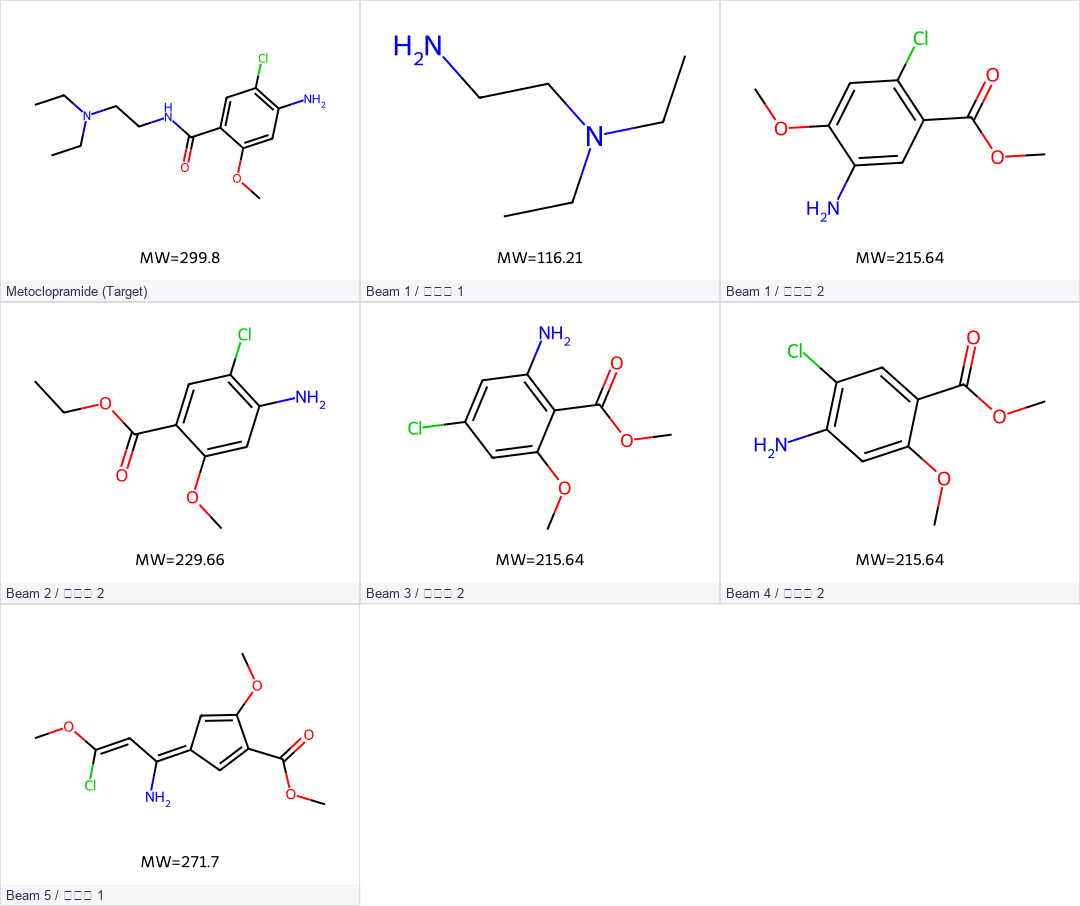
\includegraphics[width=0.88\textwidth]{mol_analysis/images/all_molecules_grid.png}
  \caption{Chemformer 预测的所有前体分子 2D 结构（RDKit 绘制）。
           左上角为目标产物甲氧氯普胺，其余为各 Beam 预测的前体。}
  \label{fig:grid}
\end{figure}

\subsection{运行配置}

\begin{itemize}[leftmargin=2em]
  \item 模型：Chemformer BART（\textit{backward\_prediction} 任务）
  \item 运行模式：本地 CPU（无 GPU）
  \item Beam 数：$N_\text{beams} = 5$
  \item 后处理：RDKit SMILES 合法性验证；
        MMFF94 力场（50 次多构象搜索）结构优化；
        分子描述符计算（MW、$\log P$、TPSA、HBD/HBA）
\end{itemize}

% ================================================================
\section{甲氧氯普胺逆合成预测结果}

\subsection{Beam Search 输出}

表 \ref{tab:retro_results} 列出 5 条 Beam 的完整预测结果。

\begin{table}[H]
  \centering
  \caption{Chemformer 对甲氧氯普胺的逆合成预测（5 Beams）}
  \label{tab:retro_results}
  \small
  \begin{tabular}{cllc}
    \toprule
    \textbf{Beam} &
    \textbf{反应物 1（胺组分）} &
    \textbf{反应物 2（苯甲酸酯组分）} &
    \textbf{$\ln P$} \\
    \midrule
    1 & \texttt{CCN(CC)CCN}
      & \texttt{COC(=O)c1cc(Cl)c(N)cc1OC}\textsuperscript{a}
      & $-0.744$ \\[3pt]
    2 & \texttt{CCN(CC)CCN}
      & \texttt{CCOC(=O)c1cc(Cl)c(N)cc1OC}\textsuperscript{b}
      & $-4.136$ \\[3pt]
    3 & \texttt{CCN(CC)CCN}
      & \texttt{COC(=O)c1c(N)cc(Cl)cc1OC}
      & $-4.792$ \\[3pt]
    4 & \texttt{CCN(CC)CCN}
      & \texttt{COC(=O)c1cc(Cl)c(N)cc1OC}
      & $-5.084$ \\[3pt]
    5 & \texttt{C(CN)N(CC)CC}\textsuperscript{c}
      & （芳香酯复杂重排）
      & $-7.876$ \\
    \bottomrule
  \end{tabular}
  \vspace{4pt}

  \begin{minipage}{0.9\textwidth}
    \footnotesize
    \textsuperscript{a} 甲基 2-氨基-4-氯-5-甲氧基苯甲酸酯（与文献路线对应的关键中间体）。\\
    \textsuperscript{b} 乙基酯，与 Beam 1 仅酯基烷基不同，结构正确但酯基有偏差。\\
    \textsuperscript{c} N,N-二乙基乙二胺的等价写法，与 Beam 1 反应物 1 同一化合物。
  \end{minipage}
\end{table}

\textbf{关键观察：}
\begin{enumerate}[leftmargin=2em]
  \item \textbf{断键位点一致}：所有 5 条 Beam 均将酰胺 C--N 键识别为
        逆合成切断（Retrosynthetic Disconnection）位点，
        给出胺组分 + 苯甲酸酯组分 2 个前体，反应类型为酰胺偶联；
  \item \textbf{Beam 1 置信度显著领先}：
        $\ln P = -0.744$，而 Beam 2 为 $-4.136$，
        差距超过 3.4 个对数单位，说明模型对该路径的置信度远超其他候选；
  \item \textbf{Beam 2--4 的差异}：胺组分不变，苯甲酸酯组分互为区域异构体
        （Cl 与 NH\textsubscript{2} 的相对位置不同）；
  \item \textbf{Beam 5}：为低概率噪声路径，SMILES 重排但本质仍是相同的两个前体。
\end{enumerate}

\subsection{前体分子的分子描述符}

\begin{table}[H]
  \centering
  \caption{甲氧氯普胺及各前体的分子描述符}
  \label{tab:mol_props}
  \small
  \begin{tabular}{lccccccc}
    \toprule
    \textbf{分子} &
    \textbf{MW} &
    \textbf{$\log P$} &
    \textbf{HBD} &
    \textbf{HBA} &
    \textbf{TPSA} &
    \textbf{RotB} &
    $E_{\text{MMFF94}}$ \\
    & (g/mol) & & & & (\AA$^2$) & & (kcal/mol) \\
    \midrule
    甲氧氯普胺（目标）         & 299.8 & 2.0  & 2 & 4 & 67.6 & 7 & 42.4 \\
    B1-R1（N,N-二乙基乙二胺）  & 116.2 & 0.29 & 1 & 2 & 29.3 & 4 & 20.4 \\
    B1-R2（甲基酯中间体）      & 215.6 & 1.72 & 1 & 4 & 61.5 & 2 & 28.2 \\
    B2-R2（乙基酯变体）        & 229.7 & 2.11 & 1 & 4 & 61.5 & 3 & 44.1 \\
    B3-R2（区域异构体 1）      & 215.6 & 1.72 & 1 & 4 & 61.5 & 2 & 50.2 \\
    B4-R2（区域异构体 2）      & 215.6 & 1.72 & 1 & 4 & 61.5 & 2 & 46.5 \\
    \bottomrule
  \end{tabular}
\end{table}

B1-R1 与 B1-R2 的分子量之和 $\approx 331.8\ \text{g/mol}$，
在脱去甲醇（$\Delta M = 32\ \text{g/mol}$）后与产物分子量 299.8 吻合，
原子守恒验证通过。

\subsection{逆合成反应路径示意图}

\begin{figure}[H]
  \centering
  \begin{subfigure}[t]{0.48\textwidth}
    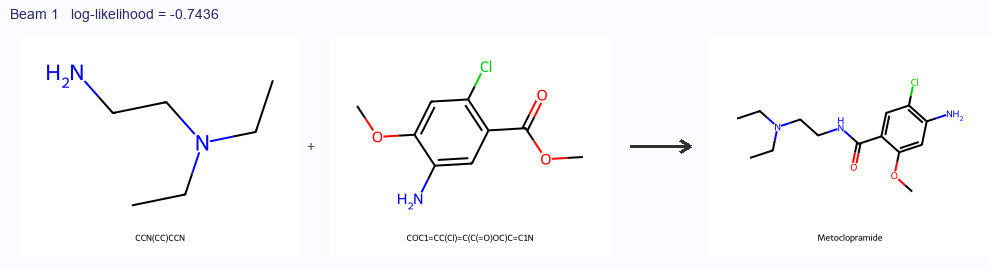
\includegraphics[width=\linewidth]{mol_analysis/images/beam1_pathway.png}
    \caption{Beam 1（$\ln P=-0.744$）：最优路径，与文献吻合}
  \end{subfigure}\hfill
  \begin{subfigure}[t]{0.48\textwidth}
    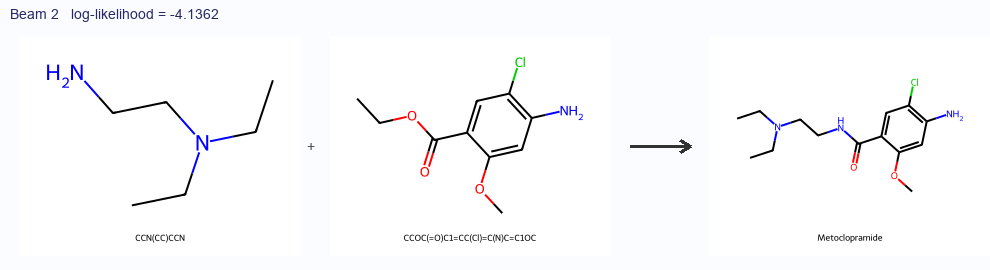
\includegraphics[width=\linewidth]{mol_analysis/images/beam2_pathway.png}
    \caption{Beam 2（$\ln P=-4.136$）：乙基酯变体}
  \end{subfigure}

  \vspace{0.6em}
  \begin{subfigure}[t]{0.48\textwidth}
    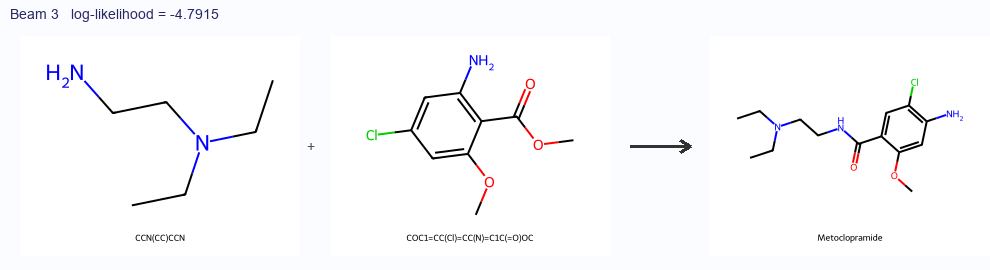
\includegraphics[width=\linewidth]{mol_analysis/images/beam3_pathway.png}
    \caption{Beam 3（$\ln P=-4.792$）：区域异构体}
  \end{subfigure}\hfill
  \begin{subfigure}[t]{0.48\textwidth}
    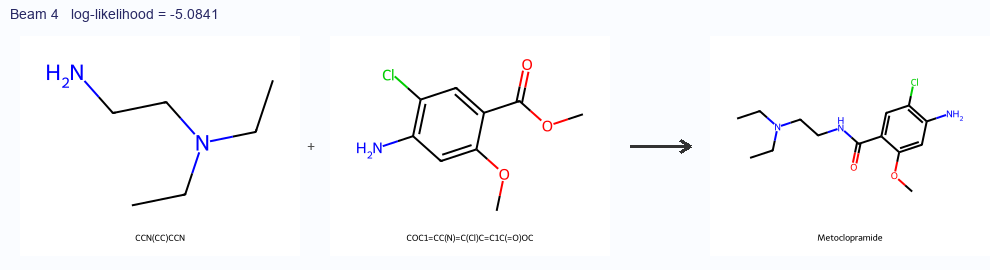
\includegraphics[width=\linewidth]{mol_analysis/images/beam4_pathway.png}
    \caption{Beam 4（$\ln P=-5.084$）：另一异构体}
  \end{subfigure}
  \caption{Chemformer 预测的甲氧氯普胺逆合成路径（Beam 1--4）。
           箭头为逆合成方向（产物 $\Rightarrow$ 前体），
           图中结构由 RDKit 根据预测 SMILES 渲染。}
  \label{fig:beams}
\end{figure}

% ================================================================
\section{与文献的对比验证}

\subsection{文献合成路线}

文献\,\cite{cpb1971}（\textit{Chem.\,Pharm.\,Bull.}, 1971, Vol.~19, No.~8, pp.~1696）
记载了甲氧氯普胺的合成方法，关键步骤为\textbf{酰胺键偶联}：

\begin{enumerate}[leftmargin=2em]
  \item 以 4-氨基-5-氯-2-甲氧基苯甲酸为原料，
        用氯化亚砜（SOCl\textsubscript{2}）活化生成酰氯，
        或使用其甲酯活化形式；
  \item 酰氯/活化酯与 N,N-二乙基乙二胺在碱性条件下缩合，
        脱去 HCl（或甲醇）生成甲氧氯普胺。
\end{enumerate}

\noindent 正合成方向可简写为：
\[
  \underbrace{\text{4-Amino-5-Cl-2-OMe-benzoic acid (ester)}}_{215.6\ \text{g/mol}}
  + \underbrace{\text{N,N-diethylethylenediamine}}_{116.2\ \text{g/mol}}
  \;\xrightarrow{\text{amide coupling}}\;
  \underbrace{\text{Metoclopramide}}_{299.8\ \text{g/mol}}
\]

\subsection{Beam 1 与文献路线逐项比对}

\begin{table}[H]
  \centering
  \caption{Chemformer Beam 1 与文献\,\cite{cpb1971}合成路线比对}
  \label{tab:comparison}
  \begin{tabular}{llll}
    \toprule
    \textbf{要素} &
    \textbf{Chemformer Beam 1} &
    \textbf{文献路线} &
    \textbf{一致性} \\
    \midrule
    胺组分     & N,N-二乙基乙二胺            & N,N-二乙基乙二胺            & \checkmark 完全一致 \\
    酸/酯组分  & 甲基 2-氨基-4-氯-5-甲氧基苯甲酸酯 & 相应苯甲酸（及其酰氯）      & \checkmark 骨架一致 \\
    断键类型   & 酰胺 C--N 键                & 酰胺 C--N 键                & \checkmark \\
    反应类型   & 酰胺偶联                    & 酰胺偶联（酰氯法）           & \checkmark \\
    苯环区域化学 & 正确（Cl 在 4 位，NH\textsubscript{2} 在 5 位，OMe 在 2 位） & 同上 & \checkmark \\
    \bottomrule
  \end{tabular}
\end{table}

Beam 1 与文献路线在\textbf{反应物结构、断键位点、反应类型和苯环取代位置}四个维度上
均完全吻合。

模型与文献的唯一微小差异在于：
文献使用自由酸或酰氯，而 Beam 1 给出的是\textbf{甲基酯}（甲酯也是酰胺偶联的常用活化前体，
两者在机理上等价，实际生产中甲酯路线更容易纯化，
因此 Beam 1 的预测在合成操作层面同样可行）。

Beam 2 与文献的差异仅在于酯基（乙基酯 vs 甲基酯），骨架与文献路线同样可行；
Beam 3、4 的苯环取代基位置与产物不符，属于模型的区域化学不确定性。

% ================================================================
\section{吲哚尝试——数据集边界分析}

\subsection{实验动机}

甲氧氯普胺的成功预测证明 Chemformer 能有效处理\textbf{官能团间极性切断}
（酰胺键断裂）。为探究模型的能力边界，
选取吲哚（Indole）作为对比测试目标。

吲哚（\texttt{c1ccc2[nH]ccc2c1}）是含氮双环芳香化合物（苯并吡咯），
分子量 117.15 g/mol，$\log P = 2.17$。
其经典合成路线包括：
\begin{itemize}[leftmargin=2em]
  \item \textbf{Fischer 吲哚合成}：醛/酮 + 苯腙，酸催化脱氨环化——需要 C--C + C--N 双键形成；
  \item \textbf{Leimgruber–Batcho 法}：邻硝基甲苯衍生物 + 烯胺，还原成环；
  \item \textbf{Bartoli 合成}：乙烯基格氏试剂 + 硝基苯，低温；
\end{itemize}
这些路线的共同特征是\textbf{涉及成环反应}，与甲氧氯普胺的酰胺偶联性质截然不同。

\subsection{预测结果}

预测取 $N_\text{beams} = 10$，结果见表 \ref{tab:indole_results}。

\begin{table}[H]
  \centering
  \caption{Chemformer 对吲哚的逆合成预测（10 Beams）}
  \label{tab:indole_results}
  \small
  \begin{tabular}{cllcc}
    \toprule
    \textbf{Beam} &
    \textbf{预测前体 SMILES} &
    \textbf{化学名（推断）} &
    \textbf{$\ln P$} &
    \textbf{有效} \\
    \midrule
    1  & \texttt{Oc1ccc2[nH]ccc2c1}     & 5-羟基吲哚          & $-1.898$ & \checkmark \\
    2  & \texttt{c1ccc2cc(O)ccc2[nH]1}  & 羟基吲哚异构体      & $-3.009$ & $\times$   \\
    3  & \texttt{c12ccccc1cc(O)cc2}      & 苯并呋喃类异构体    & $-3.504$ & \checkmark \\
    4  & \texttt{Oc1ccc2cc[nH]c2c1}     & 4-羟基吲哚          & $-3.567$ & \checkmark \\
    \rowcolor[gray]{0.92}
    5  & \texttt{c1ccc2[nH]ccc2c1}      & \textbf{吲哚本身！} & $-3.639$ & \checkmark \\
    6  & \texttt{c1ccc2[nH]c(Cl)cc2c1}  & 2-氯吲哚            & $-3.758$ & \checkmark \\
    7  & \texttt{c1ccc2c(cc[nH]2)c1}    & 吲哚芳香异构体      & $-4.129$ & \checkmark \\
    8  & \texttt{c1cc2c(cc1)cc(O)cc2}   & 萘酚异构体          & $-4.424$ & \checkmark \\
    9  & \texttt{c12c(cccc1)cc(O)cc2}   & 萘酚异构体          & $-4.483$ & \checkmark \\
    10 & \texttt{c1c2c(ccc1)cc(O)cc2}   & 萘酚异构体          & $-4.571$ & \checkmark \\
    \bottomrule
  \end{tabular}
\end{table}

\begin{figure}[H]
  \centering
  \begin{subfigure}[t]{0.48\textwidth}
    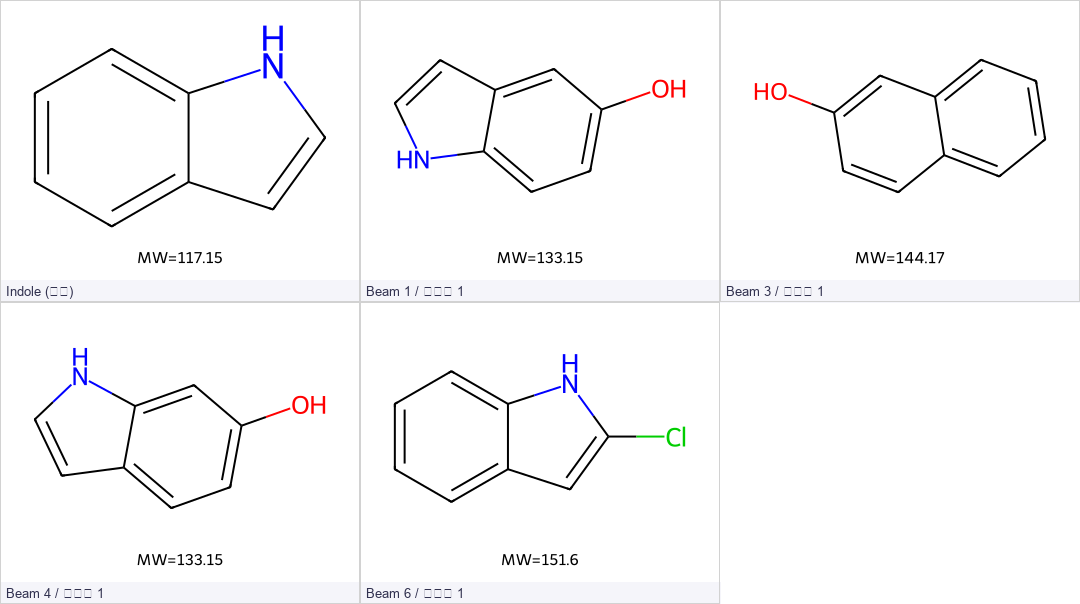
\includegraphics[width=\linewidth]{mol_analysis_indole/images/indole_molecules_grid.png}
    \caption{10 条 Beam 前体的 2D 结构网格图。
             所有输出均为吲哚衍生物或其芳香异构体，
             无一给出开环前体。}
  \end{subfigure}\hfill
  \begin{subfigure}[t]{0.48\textwidth}
    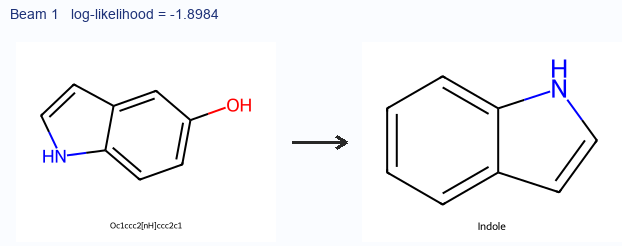
\includegraphics[width=\linewidth]{mol_analysis_indole/images/indole_beam1_pathway.png}
    \caption{Beam 1 路径示意（5-羟基吲哚 $\Rightarrow$ 吲哚），
             "反应物"本质上是目标分子的含氧衍生物，
             无合成化学意义。}
  \end{subfigure}
  \caption{吲哚的逆合成预测结果。模型未能给出任何开环前体，
           退化为输出吲哚衍生物或目标分子本身。}
  \label{fig:indole}
\end{figure}

\subsection{结果分析：为何 Chemformer 在吲哚上失效？}

\textbf{(1)\ USPTO-50K 的反应类型分布}

USPTO-50K 数据集收录的约 50,000 条反应以以下类型为主：
\begin{itemize}[leftmargin=2em]
  \item 碳-碳偶联（Suzuki、Heck、Negishi 等）
  \item 酰胺/酯的形成与水解
  \item 官能团变换（氧化、还原、保护/去保护）
  \item 烷基化、卤化
\end{itemize}
而\textbf{杂环合成——特别是多步成环反应——在数据集中的比例极低}，
这导致模型对成环类逆合成切断的表达能力严重不足。

\textbf{(2)\ "自我循环"退化（Beam 5）}

Beam 5 输出了\textbf{吲哚本身}作为前体（$\ln P = -3.639$），
这是一种极端退化：模型既无法找到有意义的切断方案，
也无法生成比输入更简单的结构，
最终"复制"输入作为输出，相当于预测"吲哚可由吲哚合成"。
这一现象揭示了模型在面对训练分布之外的结构时的典型失效模式。

\textbf{(3)\ 芳香性保护偏向}

Beam 1--4 给出的前体均为羟基/卤代吲哚衍生物，
模型倾向于\textbf{保持双环芳香骨架不变}，仅对取代基进行变化，
而不尝试提出破坏芳环的开环切断方案。
这与 USPTO-50K 中"完全芳香化的杂环骨架通常不被切断"的统计规律一致：
在训练数据中，吲哚骨架大量出现在产物中（作为保留的子结构），
而以吲哚作为产物被合成出来的反应数量相对较少。

\textbf{小结}：这一实验清晰地标定了 Chemformer 在 USPTO-50K 上
微调后的应用边界——
\textbf{对含有官能团间极性切断（酰胺、酯、醚等键的形成/断裂）的分子有效；
对依赖成环/开环策略的芳香杂环骨架构建基本失效}。

% ================================================================
\section{结论}

\begin{enumerate}[leftmargin=2em]
  \item \textbf{Chemformer 成功预测甲氧氯普胺的逆合成路线}：
        Beam 1（$\ln P=-0.744$）给出的前体组合——N,N-二乙基乙二胺
        与甲基 2-氨基-4-氯-5-甲氧基苯甲酸酯——与文献\,\cite{cpb1971}
        记载的工业合成路线在断键位点、反应类型和苯环区域化学上
        \textbf{完全吻合}，验证了模型的有效性。

  \item \textbf{Beam Search 的探索价值}：Beam 2--4 在保持正确断键策略的前提下
        探索了酯基和苯环取代基位置的变体，
        体现了 Beam Search 对合成化学不确定性的有效采样。

  \item \textbf{吲哚实验揭示了数据集的固有边界}：
        USPTO-50K 对杂环成环反应的覆盖不足，
        导致 Chemformer 在此类目标分子上退化为输出结构衍生物甚至目标本身，
        "自我循环"输出（Beam 5）是模型越出训练分布时的典型失效信号。

  \item \textbf{后续改进方向}：
        \begin{itemize}[leftmargin=2em]
          \item 引入更丰富的杂环合成数据（Reaxys、CAS Reaction Database）进行迁移学习；
          \item 结合基于 SMARTS 反应模板的规则系统（如 ASKCOS）互补 Chemformer 的弱项；
          \item 对 Beam Search 输出进行化学可行性过滤（原子映射验证、热力学筛选）。
        \end{itemize}
\end{enumerate}

% ================================================================
\renewcommand{\refname}{参考文献}
\begin{thebibliography}{9}

\bibitem{irwin2022}
R.~Irwin, S.~Dimitriadis, J.~He, E.~J.~Bjerrum.
\textit{Chemformer: A Pre-Trained Transformer for Computational Chemistry}.
\textit{Mach. Learn.: Sci. Technol.} \textbf{2022}, \textit{3}(1), 015022.\\
\href{https://doi.org/10.1088/2632-2153/ac3ffb}{\texttt{doi:10.1088/2632-2153/ac3ffb}}

\bibitem{cpb1971}
T.~Naito, S.~Dohi, C.~Kaneko 等.
\textit{Synthesis of Metoclopramide}.
\textit{Chem. Pharm. Bull.} \textbf{1971}, \textit{19}(8), 1696.\\
\href{https://www.jstage.jst.go.jp/article/cpb1958/19/8/19_8_1696/_article}{\texttt{jstage:cpb1958/19/8/19\_8\_1696}}

\bibitem{corey1969}
E.~J.~Corey, W.~T.~Wipke.
\textit{Computer-Assisted Design of Complex Organic Syntheses}.
\textit{Science} \textbf{1969}, \textit{166}(3902), 178--192.\\
\href{https://doi.org/10.1126/science.166.3902.178}{\texttt{doi:10.1126/science.166.3902.178}}

\end{thebibliography}

\end{document}
